\clearpage
\begin{flushright}
    \textit{Лекция №18}
    \textit{2015.11.17}
\end{flushright}

\section{RPC (вызов удаленных процедур)}

???
Для какой-то функции от своего имени. RPC (вызов удаленных процедур) был предложен юниксоидами и этот механизм предназначен для удаленного доступа, реализован таким образом, что вызов этой удаленной функции выполняется также как вызов локальной функции. Такое взаимодействие выполняется по схеме клиент-сервер. Процесс, вызывающий RPC, является клиентским, а процесс, который выполняет РПЦ функцию – является серверным. RPC является низкоуровневым средством взаимодействия, от этого не становится менее интересным. У RPC есть особенности, главное из которых является то, что механизм RPC скрывает от пользователя этот механизм удаленного доступа. Пользователь RPC может не заморачиваться на то, что он обращается к удаленной машине.  
РПЦ появились в 80-е. 

\begin{figure}[H]
    \centering
    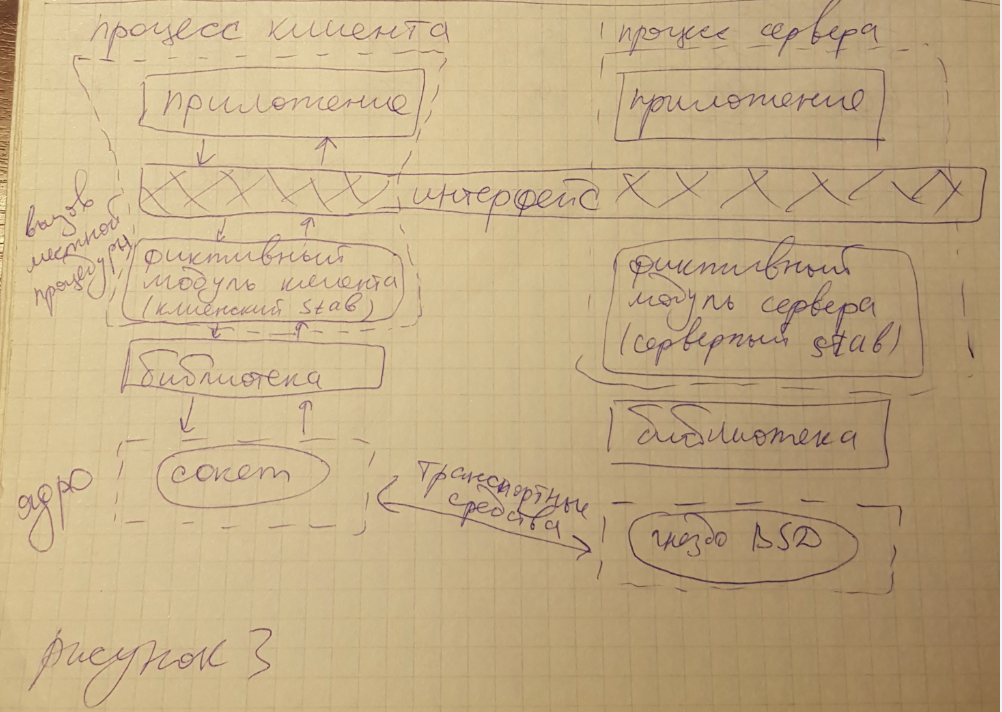
\includegraphics[width=\textwidth]{pic/3.png}
    \caption{Методология RPC}
\end{figure}

После того, как клиентский стаб (заглушка, нереальный вызов) вызван программой клиентом, Он заполняет буфер отправленным сообщением, затем параметры этого сообщения преобразуются в определенный формат и формируется пакет/несколько пакетов. После чего осуществляется переключение в режим ядра, сохраняется контекст процесса, ядро копирует сообщение/пакет в свое адресное пространство и выполняет отправку пакета серверу. На стороне сервера полученное сообщение распаковывается, ядро определяет, какому серверному стабу адресовано это сообщение. Если такой стаб на стороне сервера имеется, то выполняется копирование пакета в его буфер. После чего выполняется переключение контекста, который произошел в результате вызова серверным стабом системного вызова receive. После того, как контекст восстановлен, сообщение восстановлено серверным стабом, приложение переходит к выполнению этого запроса RPC и формирует ответное сообщение.

Проблемы, возникающие при таком взаимодействии, является указание в клиентском приложении сетевого адреса сервера. Такой подход имеет недостаток, т.е. его крайнюю не гибкость, а именно, сервер может быть перемещен или может быть увеличено число серверов, кроме того, может быть изменен интерфейс. В результате всех этих изменений необходимо заново перекомпилировать программу, которая использует жесткий адрес. Чтобы избежать такие проблемы, в некоторых распределенных системах существует динамическое связывание (биндинг).

\section{Неделимые транзакции}

Транзакция – последовательность операций над одним/несколькими объектами базы данных, которые переводят систему из одного целостное состояние в другое целостное состояние. 
Модель неделимой транзакции пришла из бизнеса. Один процесс объявляет, что хочет начать транзакцию с одним или более процессов. Инициатор транзакции объявляет, что он хочет завершить транзакцию. Если все процессы с ним соглашаются, то результат фиксируется. Если один/более процессов отказываются/потерпели крах, тогда все изменения возвращаются к исходному состоянию. 
Системные вызовы: \verb|begin|, \verb|abort|, \verb|and|, \verb|read|, \verb|write|.
Транзакции обладают свойствами упорядоченности, неделимости, постоянством.
Неделимость – промежуточные результаты не видны.

Существует два глобальных подхода к реализации неделимых транзакций:
\begin{enumerate}
    \item Создание для процессов, участвующих в транзакции, индивидуального рабочего пространства, в которых должны находиться копии всех необходимых файлов и объектов, участвующих в транзакции. Все изменения, выполняемые в процессе транзакции, выполняются в этих копиях. Исходные файлы и объекты не изменяются в процессе транзакции. Если транзакция фиксируется, то сделанные изменения копируются в исходные объекты и файлы. Недостаток: большое количество копий.
    \item Список намерений. Заключается он в том, что модифицируются сами файлы, не существует дополнительных копий. Все изменения вносятся в журнал регистрации. Там отмечается, какая транзакция делает изменение, какой файл меняется, какой блог редактируется, а так же старое и новое значения. Только после успешной записи в журнал изменяется сам файл. Если транзакция фиксируется, об этом делается запись в журнале регистрации, но старые значения все равно сохраняются. Если транзакция прерывается, то инфо из журнала используется для приведения файла в исходное состояние. В распределенных системах транзакция может потребовать взаимодействие процессов на разных машинах. На каждой машине хранятся ???. Для достижения этого в распределенных системах используется протокол двухфазной фиксации транзакций. Это самый распространённый протокол. Суть протокола: один из процессов выполняет функции координатора. Координатор начинает транзакцию и делает запись в своем локальном журнале.  После этого он посылает подчиненным процессам, участвующим в транзакции, сообщение «приготовиться».
\end{enumerate} 

\begin{figure}[H]
    \centering
    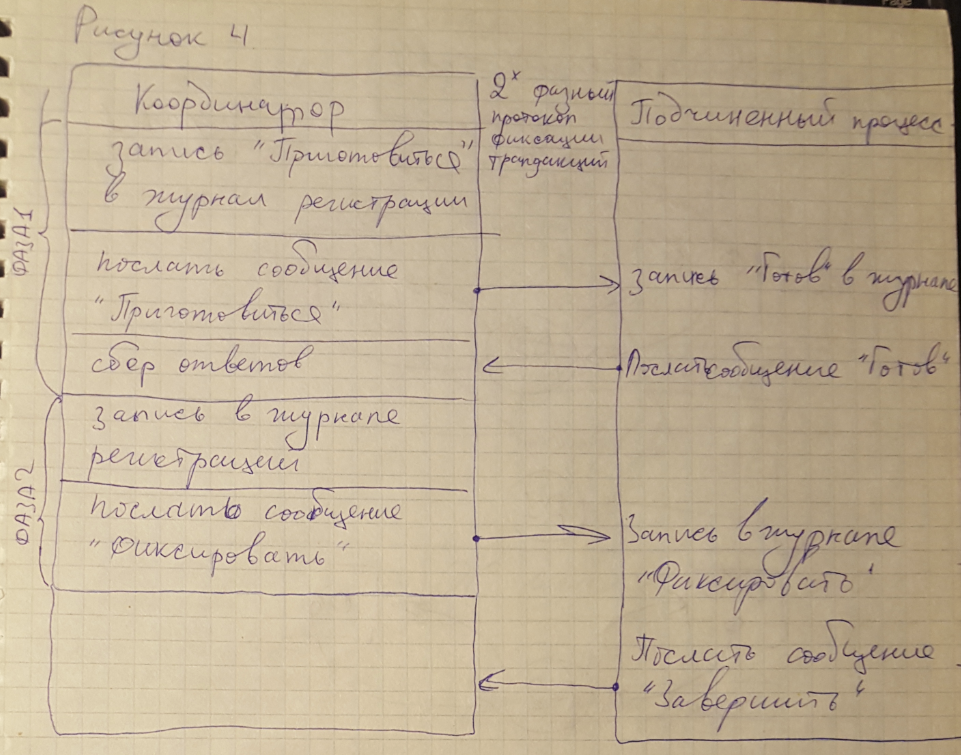
\includegraphics[width=\textwidth]{pic/4.png}
    \caption{pic}
\end{figure}

\section{Тупики}

Теория тупиков в \cite{Show_Logic_os}. Глава про тупики, автор доказывает ряд теорем, которые позволяют обнаруживать тупики.

\begin{table}[H]
\caption{Тупик}
\begin{tabular}{|l|l|}
\hline
Процесс №1 & Процесс №2 \\
\hline
Запрос ресурса Р1 & \\
Получение ресурса Р1 & \\
\hline
 & Запрос ресурса Р2\\
 & Получение ресурса Р2\\
\hline
Запрос ресурса Р2 & \\
\hline
 & Запрос ресурса Р1\\
\end{tabular}
\end{table}

Тупик – ситуация, возникающая в результате монопольного использования ресурсов, когда процесс, владея ресурсом, запрашивает другой ресурс, занятый непосредственно/через цепочку запросов процессом, который ожидает освобождения ресурсов, занятых первым процессом.

\begin{figure}[H]
    \centering
    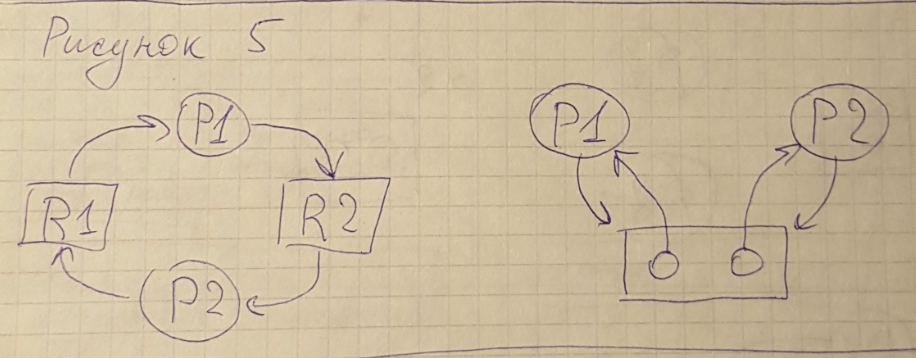
\includegraphics[width=\textwidth]{pic/5.png}
    \caption{Граф Тупика для двух единичных ресурсов}
\end{figure}

Типы ресурсов:
\begin{enumerate}
    \item потребляемые ресурсы (сообщения, когда получено, перестает существовать);
    \item повторно используемые ресурсы (аппаратные ресурсы системы, системные таблицы, реентерабельный код).
\end{enumerate} 

\begin{figure}[H]
    \centering
    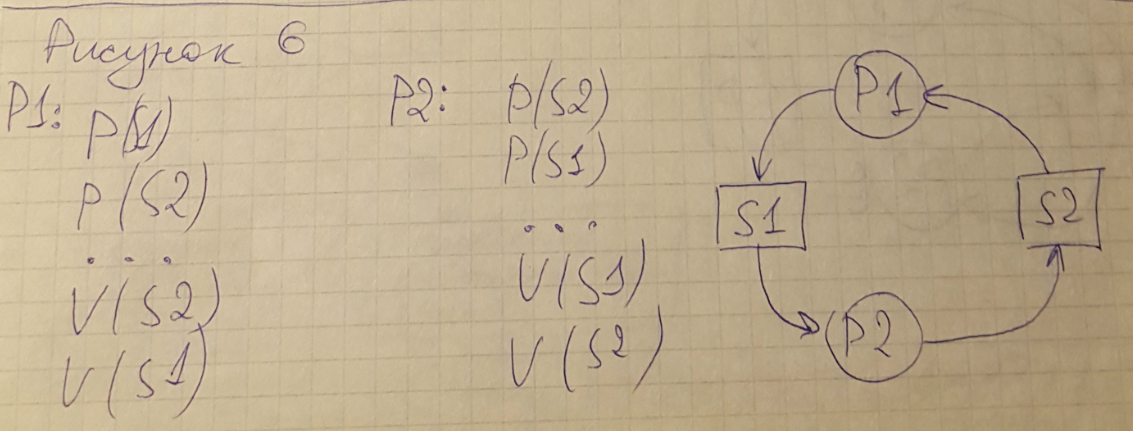
\includegraphics[width=\textwidth]{pic/6.png}
    \caption{pic}
\end{figure}

Условия возникновения тупика:
\begin{enumerate}
    \item взаимоисключение, когда процессы монопольно используют предоставляемые им ресурсы;
    \item ожидание, связано с тем, что процесс удерживает занятые им ресурсы и ожидает предоставления доп. ресурсов для возможности продолжения выполнения;
    \item неперераспределяемость, у процесса нельзя отобрать ресурсы до завершения процессов или до того момента, когда процесс сам освободит занимаемые ресурсы;
    \item круговое ожидание, возникает замкнутая цепь запросов процессов к ресурсам, в котором каждый процесс занимает ресурс, необходимый следующему процессу в цепочке, для продолжения выполнения.
\end{enumerate} 


\paragraph{Борьба с тупиками (3 метода)}

- недопущение, создание в системе такой ситуации, когда тупики в принципе невозможны. 

Одна из причин должна быть устранена. Ханвендер в своей работе доказал, что если устранить хотя бы одну причину, то тупик не возникнет. Согласно этой стратегии существует  три основных подхода:

1. Если процесс сразу запрашивает все необходимые ему ресурсы. Так было в первых системах. Бесконечное откладывание! 

2. 

- обход, тупики возможны, но в системе прикладываются усилия, чтобы их обойти;

- обнаружение тупиков, они возникают, и задача – обнаружить, а после – восстановить работоспособность системы;

- недопущение ???
